% Created by tikzDevice version 0.12
% !TEX encoding = UTF-8 Unicode
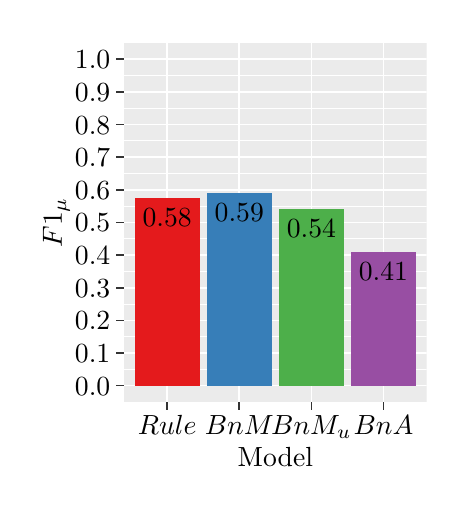
\begin{tikzpicture}[x=1pt,y=1pt]
\definecolor{fillColor}{RGB}{255,255,255}
\path[use as bounding box,fill=fillColor,fill opacity=0.00] (0,0) rectangle (149.67,166.12);
\begin{scope}
\path[clip] (  0.00,  0.00) rectangle (149.67,166.12);
\definecolor{drawColor}{RGB}{255,255,255}
\definecolor{fillColor}{RGB}{255,255,255}

\path[draw=drawColor,line width= 0.6pt,line join=round,line cap=round,fill=fillColor] (  0.00,  0.00) rectangle (149.67,166.12);
\end{scope}
\begin{scope}
\path[clip] ( 34.81, 30.86) rectangle (144.17,160.62);
\definecolor{fillColor}{gray}{0.92}

\path[fill=fillColor] ( 34.81, 30.86) rectangle (144.17,160.62);
\definecolor{drawColor}{RGB}{255,255,255}

\path[draw=drawColor,line width= 0.3pt,line join=round] ( 34.81, 42.66) --
	(144.17, 42.66);

\path[draw=drawColor,line width= 0.3pt,line join=round] ( 34.81, 54.45) --
	(144.17, 54.45);

\path[draw=drawColor,line width= 0.3pt,line join=round] ( 34.81, 66.25) --
	(144.17, 66.25);

\path[draw=drawColor,line width= 0.3pt,line join=round] ( 34.81, 78.05) --
	(144.17, 78.05);

\path[draw=drawColor,line width= 0.3pt,line join=round] ( 34.81, 89.84) --
	(144.17, 89.84);

\path[draw=drawColor,line width= 0.3pt,line join=round] ( 34.81,101.64) --
	(144.17,101.64);

\path[draw=drawColor,line width= 0.3pt,line join=round] ( 34.81,113.43) --
	(144.17,113.43);

\path[draw=drawColor,line width= 0.3pt,line join=round] ( 34.81,125.23) --
	(144.17,125.23);

\path[draw=drawColor,line width= 0.3pt,line join=round] ( 34.81,137.03) --
	(144.17,137.03);

\path[draw=drawColor,line width= 0.3pt,line join=round] ( 34.81,148.82) --
	(144.17,148.82);

\path[draw=drawColor,line width= 0.6pt,line join=round] ( 34.81, 36.76) --
	(144.17, 36.76);

\path[draw=drawColor,line width= 0.6pt,line join=round] ( 34.81, 48.56) --
	(144.17, 48.56);

\path[draw=drawColor,line width= 0.6pt,line join=round] ( 34.81, 60.35) --
	(144.17, 60.35);

\path[draw=drawColor,line width= 0.6pt,line join=round] ( 34.81, 72.15) --
	(144.17, 72.15);

\path[draw=drawColor,line width= 0.6pt,line join=round] ( 34.81, 83.94) --
	(144.17, 83.94);

\path[draw=drawColor,line width= 0.6pt,line join=round] ( 34.81, 95.74) --
	(144.17, 95.74);

\path[draw=drawColor,line width= 0.6pt,line join=round] ( 34.81,107.54) --
	(144.17,107.54);

\path[draw=drawColor,line width= 0.6pt,line join=round] ( 34.81,119.33) --
	(144.17,119.33);

\path[draw=drawColor,line width= 0.6pt,line join=round] ( 34.81,131.13) --
	(144.17,131.13);

\path[draw=drawColor,line width= 0.6pt,line join=round] ( 34.81,142.92) --
	(144.17,142.92);

\path[draw=drawColor,line width= 0.6pt,line join=round] ( 34.81,154.72) --
	(144.17,154.72);

\path[draw=drawColor,line width= 0.6pt,line join=round] ( 50.43, 30.86) --
	( 50.43,160.62);

\path[draw=drawColor,line width= 0.6pt,line join=round] ( 76.47, 30.86) --
	( 76.47,160.62);

\path[draw=drawColor,line width= 0.6pt,line join=round] (102.51, 30.86) --
	(102.51,160.62);

\path[draw=drawColor,line width= 0.6pt,line join=round] (128.55, 30.86) --
	(128.55,160.62);
\definecolor{fillColor}{RGB}{228,26,28}

\path[fill=fillColor] ( 38.71, 36.76) rectangle ( 62.15,104.72);
\definecolor{fillColor}{RGB}{55,126,184}

\path[fill=fillColor] ( 64.75, 36.76) rectangle ( 88.19,106.46);
\definecolor{fillColor}{RGB}{77,175,74}

\path[fill=fillColor] ( 90.79, 36.76) rectangle (114.23,100.50);
\definecolor{fillColor}{RGB}{152,78,163}

\path[fill=fillColor] (116.83, 36.76) rectangle (140.27, 85.07);
\definecolor{drawColor}{RGB}{0,0,0}

\node[text=drawColor,anchor=base,inner sep=0pt, outer sep=0pt, scale=  1.00] at (128.55, 74.69) {0.41};

\node[text=drawColor,anchor=base,inner sep=0pt, outer sep=0pt, scale=  1.00] at (102.51, 90.13) {0.54};

\node[text=drawColor,anchor=base,inner sep=0pt, outer sep=0pt, scale=  1.00] at ( 76.47, 96.09) {0.59};

\node[text=drawColor,anchor=base,inner sep=0pt, outer sep=0pt, scale=  1.00] at ( 50.43, 94.35) {0.58};
\end{scope}
\begin{scope}
\path[clip] (  0.00,  0.00) rectangle (149.67,166.12);
\definecolor{drawColor}{RGB}{0,0,0}

\node[text=drawColor,anchor=base east,inner sep=0pt, outer sep=0pt, scale=  1.00] at ( 29.86, 33.32) {0.0};

\node[text=drawColor,anchor=base east,inner sep=0pt, outer sep=0pt, scale=  1.00] at ( 29.86, 45.11) {0.1};

\node[text=drawColor,anchor=base east,inner sep=0pt, outer sep=0pt, scale=  1.00] at ( 29.86, 56.91) {0.2};

\node[text=drawColor,anchor=base east,inner sep=0pt, outer sep=0pt, scale=  1.00] at ( 29.86, 68.70) {0.3};

\node[text=drawColor,anchor=base east,inner sep=0pt, outer sep=0pt, scale=  1.00] at ( 29.86, 80.50) {0.4};

\node[text=drawColor,anchor=base east,inner sep=0pt, outer sep=0pt, scale=  1.00] at ( 29.86, 92.30) {0.5};

\node[text=drawColor,anchor=base east,inner sep=0pt, outer sep=0pt, scale=  1.00] at ( 29.86,104.09) {0.6};

\node[text=drawColor,anchor=base east,inner sep=0pt, outer sep=0pt, scale=  1.00] at ( 29.86,115.89) {0.7};

\node[text=drawColor,anchor=base east,inner sep=0pt, outer sep=0pt, scale=  1.00] at ( 29.86,127.68) {0.8};

\node[text=drawColor,anchor=base east,inner sep=0pt, outer sep=0pt, scale=  1.00] at ( 29.86,139.48) {0.9};

\node[text=drawColor,anchor=base east,inner sep=0pt, outer sep=0pt, scale=  1.00] at ( 29.86,151.28) {1.0};
\end{scope}
\begin{scope}
\path[clip] (  0.00,  0.00) rectangle (149.67,166.12);
\definecolor{drawColor}{gray}{0.20}

\path[draw=drawColor,line width= 0.6pt,line join=round] ( 32.06, 36.76) --
	( 34.81, 36.76);

\path[draw=drawColor,line width= 0.6pt,line join=round] ( 32.06, 48.56) --
	( 34.81, 48.56);

\path[draw=drawColor,line width= 0.6pt,line join=round] ( 32.06, 60.35) --
	( 34.81, 60.35);

\path[draw=drawColor,line width= 0.6pt,line join=round] ( 32.06, 72.15) --
	( 34.81, 72.15);

\path[draw=drawColor,line width= 0.6pt,line join=round] ( 32.06, 83.94) --
	( 34.81, 83.94);

\path[draw=drawColor,line width= 0.6pt,line join=round] ( 32.06, 95.74) --
	( 34.81, 95.74);

\path[draw=drawColor,line width= 0.6pt,line join=round] ( 32.06,107.54) --
	( 34.81,107.54);

\path[draw=drawColor,line width= 0.6pt,line join=round] ( 32.06,119.33) --
	( 34.81,119.33);

\path[draw=drawColor,line width= 0.6pt,line join=round] ( 32.06,131.13) --
	( 34.81,131.13);

\path[draw=drawColor,line width= 0.6pt,line join=round] ( 32.06,142.92) --
	( 34.81,142.92);

\path[draw=drawColor,line width= 0.6pt,line join=round] ( 32.06,154.72) --
	( 34.81,154.72);
\end{scope}
\begin{scope}
\path[clip] (  0.00,  0.00) rectangle (149.67,166.12);
\definecolor{drawColor}{gray}{0.20}

\path[draw=drawColor,line width= 0.6pt,line join=round] ( 50.43, 28.11) --
	( 50.43, 30.86);

\path[draw=drawColor,line width= 0.6pt,line join=round] ( 76.47, 28.11) --
	( 76.47, 30.86);

\path[draw=drawColor,line width= 0.6pt,line join=round] (102.51, 28.11) --
	(102.51, 30.86);

\path[draw=drawColor,line width= 0.6pt,line join=round] (128.55, 28.11) --
	(128.55, 30.86);
\end{scope}
\begin{scope}
\path[clip] (  0.00,  0.00) rectangle (149.67,166.12);
\definecolor{drawColor}{RGB}{0,0,0}

\node[text=drawColor,anchor=base,inner sep=0pt, outer sep=0pt, scale=  1.00] at ( 50.43, 19.03) {\(Rule\)};

\node[text=drawColor,anchor=base,inner sep=0pt, outer sep=0pt, scale=  1.00] at ( 76.47, 19.03) {\(BnM\)};

\node[text=drawColor,anchor=base,inner sep=0pt, outer sep=0pt, scale=  1.00] at (102.51, 19.03) {\(BnM_u\)};

\node[text=drawColor,anchor=base,inner sep=0pt, outer sep=0pt, scale=  1.00] at (128.55, 19.03) {\(BnA\)};
\end{scope}
\begin{scope}
\path[clip] (  0.00,  0.00) rectangle (149.67,166.12);
\definecolor{drawColor}{RGB}{0,0,0}

\node[text=drawColor,anchor=base,inner sep=0pt, outer sep=0pt, scale=  1.00] at ( 89.49,  7.44) {Model};
\end{scope}
\begin{scope}
\path[clip] (  0.00,  0.00) rectangle (149.67,166.12);
\definecolor{drawColor}{RGB}{0,0,0}

\node[text=drawColor,rotate= 90.00,anchor=base,inner sep=0pt, outer sep=0pt, scale=  1.00] at ( 12.39, 95.74) {\(F1_\mu\)};
\end{scope}
\end{tikzpicture}
